%% ---------------------------------------------------------------------------
%% Thesis.tex -- MAIN FILE (the one that you compile with LaTeX)
%% ---------------------------------------------------------------------------
% https://www.sharelatex.com/templates/thesis/graduate-thesis/
% Set up the document
% Use the "Thesis" style, based on the ECS Thesis style by Steve Gunn
% use the draft option to print overfull hbox
\documentclass[a4paper, 11pt, oneside]{Thesis}
% : change to twosize when done
%\documentclass[a4paper, 11pt, twoside]{Thesis}
% Location of the graphics files (set up for graphics to be in PDF format)
\graphicspath{Figures/}

% Include any extra LaTeX packages required
% Use biblatex to bibliography management
\usepackage[
  backend=biber,
  style=numeric,
  sorting=ynt,
  hyperref=true,
  maxbibnames=15,
  maxcitenames=3,
]{biblatex}
\addbibresource{Bibliography.bib}
% Needed for the "comment" environment to make LaTeX comments
\usepackage{verbatim}
% Allows "\bvec{}" and "\buvec{}" for "blackboard" style bold vectors in maths
\usepackage{vector}
% Todos
\usepackage{todonotes}
% set default todo style to fancyline
\presetkeys{todonotes}{fancyline,size=\tiny}{}
% Todonotes wrongly placed in the margin
%TODO: remove this by the end?
\setlength{\marginparwidth}{2cm}

% indent description lists
%\usepackage{enumitem}
%\setdescription{leftmargin=\parindent,labelindent=\parindent}

%\usepackage[utf8]{inputenc}
% Colour hyperlinks in blue, but this can be distracting if there are many
% links.
\hypersetup{urlcolor=blue, colorlinks=false}
% show frames around the margins
%\usepackage[showframe,pass]{geometry}
% nomenclature and glossary
\usepackage[norefpage]{nomencl}
\renewcommand{\nomname}{Abbreviations}
% Abbreviation in bold
\renewcommand{\nomlabel}[1]{\textbf{#1}}
% no extra skip between entries
\setlength{\nomitemsep}{-\parsep}
% costumize the rightmark and leftmark from fancyhdr
\renewcommand{\chaptermark}[1]{ \markboth{\MakeUppercase{\thechapter.\ #1}}{}}
\renewcommand{\sectionmark}[1]{ \markright{\thesection.\ #1}{ }}

\makenomenclature

\usepackage{comment}


% gantt diagram
\usepackage{pgfgantt}

% include new commands
\usepackage{Commands}
\usepackage{pdfpages}

%% ---------------------------------------------------------------------------
\begin{document}
%\includepdf[pages={1}]{parecer.pdf}

% Begin Roman style (i, ii, iii, iv...) page numbering
\frontmatter

% Set up the Title Page
\title  {Distributed Aggregation Algorithms in Smart Meters
        \\[1.5cm]\large{Pre-Dissertation Report}}
\authors  {\texorpdfstring
            {\href{mailto:rafael.remondes@gmail.com}{Telmo Rafael Rodriges Remondes}}
            {Rafael Remondes}
            }
% Do not change this here, instead these must be set in the "Thesis.cls" file,
% please look through it instead
\addresses  {\groupname\\\deptname\\\univname}
\date       {\today}
\subject    {}
\keywords   {}

\maketitle
%% ---------------------------------------------------------------------------

% It is better to have smaller font and larger line spacing than the other way
% round
\setstretch{1.5}

% Define the page headers using the FancyHdr package and set up for one-sided
% printing
% Clears all page headers and footers
\fancyhead{}
% Sets the right side header to show the page number
\rhead{\thepage}
% Clears the left side page header
\lhead{}

% Finally, use the "fancy" page style to implement the FancyHdr headers
\pagestyle{fancy}

%% ---------------------------------------------------------------------------
%% Declaration Page required for the Thesis, your institution may give you
%% a different text to place here
%\Declaration{
%
%% Add a gap in the Contents, for aesthetics
%\addtocontents{toc}{\vspace{1em}}
%
%I, AUTHOR NAME, declare that this thesis titled, `THESIS TITLE' and the work
%presented in it are my own. I confirm that:
%
%\begin{itemize} 
%\item[\tiny{$\blacksquare$}] This work was done wholly or mainly while in
%  candidature for a research degree at this University.
% 
%\item[\tiny{$\blacksquare$}] Where any part of this thesis has previously been
%  submitted for a degree or any other qualification at this University or any
%  other institution, this has been clearly stated.
% 
%\item[\tiny{$\blacksquare$}] Where I have consulted the published work of
%  others, this is always clearly attributed.
% 
%\item[\tiny{$\blacksquare$}] Where I have quoted from the work of others, the
%  source is always given. With the exception of such quotations, this thesis is
%  entirely my own work.
% 
%\item[\tiny{$\blacksquare$}] I have acknowledged all main sources of help.
% 
%\item[\tiny{$\blacksquare$}] Where the thesis is based on work done by myself
%  jointly with others, I have made clear exactly what was done by others and
%  what I have contributed myself.
%\\
%\end{itemize}
% 
% 
%Signed:\\
%% This prints a line for the signature
%\rule[1em]{25em}{0.5pt}
% 
%Date:\\
%% This prints a line to write the date
%\rule[1em]{25em}{0.5pt}
%}
%% Declaration ended, now start a new page
%\clearpage
%
%% ---------------------------------------------------------------------------
% The "Funny Quote Page"
% No headers or footers for the following pages
%\pagestyle{empty}
%
%\null\vfill
%% Now comes the "Funny Quote", written in italics
%\textit{``Write a funny quote here.''}
%
%\begin{flushright}
%If the quote is taken from someone, their name goes here
%\end{flushright}
%
%\vfill\vfill\vfill\vfill\vfill\vfill\null
%\clearpage  % Funny Quote page ended, start a new page
%% ---------------------------------------------------------------------------

% The Abstract Page
% Add the "Abstract" page entry to the Contents
\addtotoc{Abstract}
\abstract{
% Add a gap in the Contents, for aesthetics
\addtocontents{toc}{\vspace{1em}}

\chapter*{Abstract}
 The power grids all over the planet become increasingly bigger leading to problems of energy waste and sustainability. Since the recognition of this kind of problems, new renewable energy resource emerge , as well as the need to integrate them into the grid. The Smart Grids show up to integrate all these new energy sources and to respond to the new demands of the modern grid. \\
This new grid is a complex system that englobes a new mechanism to collect measurement data from the consumers meters. The new meters, the smart meters, along with the smart metering system enable the overall system to collect fine-granular readings regarding the energy consumed by the costumers. With the aggregation of this data, several other goals could be achieved such as time-adaptive tariffs, load balancing the distribution of energy and saving computation resources since the aggregation enables to summarize the collected data.\\
In this work we address the problem of smart metering data aggregation. We propose a distributed data aggregation approach, where all the smart meter sense the consumption data and some of them can work as aggregators as well. We also focus in observing how the aggregation algorithms work in the smart grid, collecting the results and evaluating which algorithm suites best.

	\cleardoublepage

\chapter*{Resumo}
	As redes eléctricas por todo o mundo tornaram-se cada vez maiores, levando a problemas de desperdício de recursos e de sustentabilidade. Desde a constatação destes problemas, novas energias  renováveis apareceram assim como a necessidade de as integrar dentro da rede. As \textit{Smart Grids} apareceram para fazer face a essa necessidade de integração e para responder as necessidade da rede moderna.\\
	A nova rede é um complexo sistema que engloba novos mecanismos para recolher dados das medições dos contadores dos consumidores. Este novos contadores, \textit{smart meters}, assim como o sistema inteligente de medição permitem a todo o sistema colecionar dados de leituras de fina granulação acerca da energia consumida pelos consumidores. Com a agregação dos dados vários outros objetivos podem ser atingidos como tarifas adaptáveis ao longo do tempo, balancear a distribuição de energia e poupar recursos computacionais considerando que a agregação permite sumariar os dados recolhidos.\\
	Neste trabalho sera tratado o problema da agregação de dados de forma distribuída.  E proposta uma abordagem distribuída de agregação, onde todos os leitores inteligentes leem o consumo de energia e alguns funcionam como agregadores.



}

% Abstract ended, start a new page
\clearpage
%% ---------------------------------------------------------------------------

%% Reset the line-spacing to 1.5 for body text (if it has changed)
%\setstretch{1.5}
%
%% The Acknowledgements page, for thanking everyone
%\acknowledgements{
%% Add a gap in the Contents, for aesthetics
%\addtocontents{toc}{\vspace{1em}}
%
%The acknowledgements and the people to thank go here, don't forget to include
%your project advisor\ldots
%
%}
%% End of the Acknowledgements
%\clearpage
%% ---------------------------------------------------------------------------

% The page style headers have been "empty" all this time, now use the "fancy"
% headers as defined before to bring them back
\pagestyle{fancy}

%% ---------------------------------------------------------------------------
% Set the left side page header to "Contents"
\lhead{\emph{Contents}}
% Write out the Table of Contents
\tableofcontents

%% ---------------------------------------------------------------------------
% Set the left side page header to "List if Figures"
\lhead{\emph{List of Figures}}
%% Write out the List of Figures
\listoffigures

%% ---------------------------------------------------------------------------
% Set the left side page header to "List of Tables"
%\lhead{\emph{List of Tables}}
%% Write out the List of Tables
%\listoftables

%% ---------------------------------------------------------------------------
% Set the line spacing to 1.5, this makes the following tables easier to read
\setstretch{1.5}
% Start a new page
\clearpage
% Set the left side page header to "Abbreviations"
\lhead{\emph{Abbreviations}}
% Include a list of Abbreviations (a table of two columns)
%\listofsymbols{ll}
%{
% \textbf{Acronym} & \textbf{W}hat (it) \textbf{S}tands \textbf{F}or \\
%\textbf{LAH} & \textbf{L}ist \textbf{A}bbreviations \textbf{H}ere \\

%}
\printnomenclature

%% ---------------------------------------------------------------------------
%% Start a new page
%\clearpage
%% Set the left side page header to "Physical Constants"
%\lhead{\emph{Physical Constants}}
%% Include a list of Physical Constants (a four column table)
%\listofconstants{lrcl}
%{
%% Constant Name & Symbol & = & Constant Value (with units) \\
%Speed of Light & $c$ & $=$ & $2.997\ 924\ 58\times10^{8}\
%\mbox{ms}^{-\mbox{s}}$ (exact)\\
%
%}

%% ---------------------------------------------------------------------------
%% Start a new page
%\clearpage
%% Set the left side page header to "Symbols"
%\lhead{\emph{Symbols}}
%% Include a list of Symbols (a three column table)
%\listofnomenclature{lll}
%{
%  % symbol & name & unit \\
%  $a$ & distance & m \\
%  $P$ & power & W (Js$^{-1}$) \\
%  & & \\ % Gap to separate the Roman symbols from the Greek
%  $\omega$ & angular frequency & rads$^{-1}$ \\
%}
%% ---------------------------------------------------------------------------
%% End of the pre-able, contents and lists of things
%% Begin the Dedication page
%\clearpage
%
%% Return the line spacing back to 1.5
%\setstretch{1.5}
%
%% Page style needs to be empty for this page
%\pagestyle{empty}
%\dedicatory{For/Dedicated to/To my\ldots}
%
%% Add a gap in the Contents, for aesthetics
%\addtocontents{toc}{\vspace{2em}}

%% ---------------------------------------------------------------------------
% Begin normal, numeric (1,2,3...) page numbering
\mainmatter

% Return the page headers back to the "fancy" style
\pagestyle{fancy}
% Clears all page headers and footers
\fancyhead{}
\fancyhead[LE,RO]{\thepage}
\fancyhead[RE]{\emph{\leftmark}}
\fancyhead[LO]{\emph{\rightmark}}
% Include the chapters of the thesis, as separate files
% Just uncomment the lines as you write the chapters

%\listoftodos

\chapter{Introduction}\label{c:intro}
The power electrical grid is a very important infrastructure in the modern world. The energy it provides is considered of main importance and a basic condition to guarantee minimum life quality. As important as it is and thanks to its large size, the power grid consumes a enormous amount of natural resources, make it unsustainable in long term. The dawn of new renewable energy sources also increase the need to modernize the grid since it's mandatory to interconnect them to the traditional Grid. The introduction of ICT and computation in the grid is trying to change it to became more sophisticated, eco sustainable and integrate all the energy sources to enable efficient electrical power distribution. This new concept of grid is called Smart Grid (\nom{SG}{Smart Grid}).

SG is a modern power grid that uses computation, information and communication. In an automatic way, SG improves the energy efficiency, sustainability both in power distribution and in electricity production. It enables the grid to become more sustainable as it makes a more efficient management of  natural resources. The SG is composed by 'Islands of Automation' interconnected with a communication infrastructure \cite{Ericsson_2}. 

Smart Meters ((\nom{SM}{Smart Meters}) are one of the main components of the Smart Grid. They are devices located in the consumers/costumers houses or in industrial facilities that sense the energy consumption. They  read periodically in short intervals that range from minutes to milliseconds. This amount of data can be used for performing statistical analyses that lead to effective consumption forecasting and profiling. This fine grained readings will assist users in achieving a more efficient energy use and adapting to the network status and supply by choosing an appropriate and advantageous tariff \cite{journals/spm/ErkinTLP13}.

In the next years, the amount of user data collected by the SG is expected to dramatically increase with respect to the current electrical power grid.The amount of \textit{Big Data} collected is important because it leads to a great number of comercial advantages and better energy consumption predictions\cite{INDIN2013aggregationPerformance}.

In this work, we look at the information collected within the SG. More specifically, the information collected by Smart Meters in the households. This data is very important, not only for billing purposes but also to improve the energy management enabling it to become more \textit{Smart}.  

\section{Objectives}
\todo{Are the Objectives clear enough?}
There are two types of architectures\cite{journals/spm/ErkinTLP13} regarding the SM data aggregation namely  \textit{decentralized} and \textit{centralized}. In a \textit{centralized} architecture, the meters only sense the energy consumption every specific time and send it to a central data aggregator center. In a \textit{decentralized} architecture the meters sense the consumers consumption too. They also perform a partial data aggregation themselves, it's called in-network aggregation\cite{journals/spm/ErkinTLP13}.

In this work, we will focus on the second type of architecture which provides more interesting challenges. The purpose of this work is, considering a \textit{decentralized} architecture, evaluate an efficient data aggregation algorithm that provides relevant information to the consumer and to the electricity producer. 
In order to achieve the main goal, it's important to first understand the various possible \textit{decentralized} architectures and the the role of each component. As  we saw in \cite{Girao2004c} there are some sensors that work as aggregation nodes an others that work as simple nodes. 

At first, it is important to know how the SG works, how all components work together in a integrated way and the status of deployed models . Furthermore, it is important to construct a suitable topology for this work, with several meters collecting information about the consumers consumption and aggregate that data in a distributed way. This topology may be constructed consedering real and deployed examples of a smart mettering system. This is an important part of this work as the study of the existed algorithm to performe distributed aggregation.

The study of distributed aggregation algorithms embraces the awareness of their functionalities, advantages and disadvantages. It also requires a implementation of then in familiar topologies to understand in better way how the algorithms behave and also to adquire insight about them. 

When we have both the topology and also the algorithms, the next step will be implement them. We are interested in knowing which algorithm provides the best results in time, exchange messages, scalability, resilience, fault tolerence and accuracy. It is also imporant to understand which aggregation funtions are important to compute in this specific context. Function such as $AVERAGE$ or $SUM$ may be important, so it is mandatory to choose algrotihm that enable these functions.

In the end, an overall comparison between the algorithms will be presented. Improvements to the algorithms may be required in order to obtain relevant information to the consumer and to the electricity producer. The improvements will occur as we select the kind of data that is important to aggregate and collect.

\section{Motivation}
\todo{Maybe some more motivation}
As stated before, Smart Grid is a new and important concept of grid that is of main importance towards the world energy sustainability. Also, the new needs and urges for integration of the new renewable energy sources make the upgrade of the grid mandatory.\\
With this concept in mind, an important part of this intelligent grid is studied. The data collected from the meters is one of the main parts of a electrical grid. Not only for billing purposes, as it is said in above section, but to achieve better management(management that enables the grid to spare less resources). Grid management could not be done as long as there is no info about the consumption.\\
The aggregation is a vital process. Aggregation summarize the overall collected data, reducing the computational power required to process the information. Doing this in a distributed fashion withdraws the need of a central aggregator with a high processing power. It also enables the aggregation to be more resilient, reliable and fault tolerant since it is distributed and  cheaper in therms of resources.


\section{Document structure}\label{s:struct}
In this document, a state of the art regarding the overall work thematic is presented. In chapter \ref{chap:sg} it is presented the various definitions of the new grid and the point they converge. It is detailed also the infrastructure and model, how the Smart grid is organized and how the diferente components interact.  The communication structure and the technologies used on it is also presented, with the various alternatives to realize communication in the modern grid. The important part for this work, smart meters, is detailed.\\
In chapter \ref{chap:wsn} is the definition of \textit{Wireless Sensor Networks}(\nom{WSN}{Wireless Sensor Network}). Smart Metering System could be consider as a specific implementation of WSN so it is important to understand how WSN work and, more important, how in-network aggregation takes place. Awareness of this aspects is important considering it's helpful to understand aggregation in Smart Metering Systems. WSN are a concept widely study with similarities with Smart Metering, a bridge between the two concepts are also presented. Although very similar,  the two networks have their differences that are presented in the same chapter.\\
In chapter \ref{chap:dda} it is referenced the concept of distributed aggregation, some aggregation function and its proprieties.  The various aggregation algorithms are referenced with its description. The distributed aggregation within  the \textit{smart meters} and WSN is mentioned as well.


 % Introduction

\chapter{Smart Grid}\label{chap:sg}
The Smart Grid  is a new concept of grid which introduces new technologies into the traditional power system. They enable power grids to become more efficient, integrate other sources of energy rather than traditional ones, and  they increase the overall management performance by using modern information technologies. The SG is capable of delivering power in more efficient way and respond to a wide variety of condition and events \cite{journals/comsur/FangMXY12}. Although there are no SGs fully implemented, there are several SG pilot projects  show that the new generation grid pose new opportunities and challenges to both consumers and producers. \\
There are several definitions for the SG among the literature. For example \cite{journals/comsur/FangMXY12} states that  "\textit{SG can be regarded as an electric system that uses information, two-way and cyber-secure communication technologies and computational intelligence in an integrated fashion to achieve a clean, safe, secure, reliable, resilient, efficient and sustainable system}".\cite{conf/isgt/GhoshPR13} considers the SG as "\textit{a platform that embraces several multidisciplinary concepts towards computerization of electrical power grids}". The common concept over the literature is that SG main goal is to integrate several components, traditional and new, to achieve better performance, interoperability, energy management and sustainability in long term. \\
SG creates an environment that introduces a convergence between the infrastructure of generation, transmission, distribution, energy, information technology and digital communication infrastructure that enables the exchange of information and control action among the various segments of the power grid.\\
As it is possible to notice, these integration means that the SG itself is a very complicated system. Achieving the mentioned goals is a complex task. Due to its variety of problems and challenges, most of the proposed solution and studies regarding the SG focus in some specific aspects. 
An interesting table that presents a comparison between the traditional grid and the SG is presented in \cite{journals/comsur/FangMXY12}:
\begin{figure}[h]
\centering
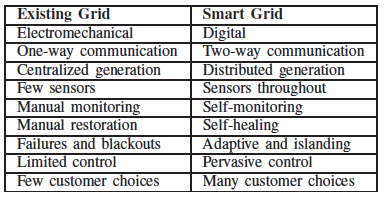
\includegraphics[width=0.5\textwidth]{/Users/rafaelremondes/UM/MEI/Thesis/DistributedAggregationAlgortihmsSM/Writing/Images/differencesTraditionalSmart}
\caption{\label{fig:comparisonOldNew} Brief Comparison Between the Existing Grid and the Smart Grid}
\end{figure}

\section{Smart Grid Model}
 The  SG  proposes a new model to the power grid where consumers are no longer passive actors in the grid, but prosumers(insert quote) that can both consume and produce energy in small quantities thanks to the new renewable energy sources, plus the introduction of ICT that means new actors that are now present in the grid, enabling new features into the traditional ones.\\
 Typically, the components in a power grid go one way, in the in SG  all the flows of electricity and information go two-ways.  These new features enable the operations to become  faster and more accurate and the interactions between them  are increased resulting that, in the future, everything that happens in the grid can be monitored almost in real time.\\
 In am ideal scenario, the SG's new vision, states that a specific component of the grid, such as a household, can both receive energy from the global grid and in the next moment can disconnect from it and become self-sustainable. \\
There are several visions and models proposed to the SG. One of the more general and accepted model, based on this vision of actors and their interactions, is  the NIST report \cite{government2011nist} which proposes a conceptual model providing the main actors towards the SG.
\begin{figure}[h]
\centering
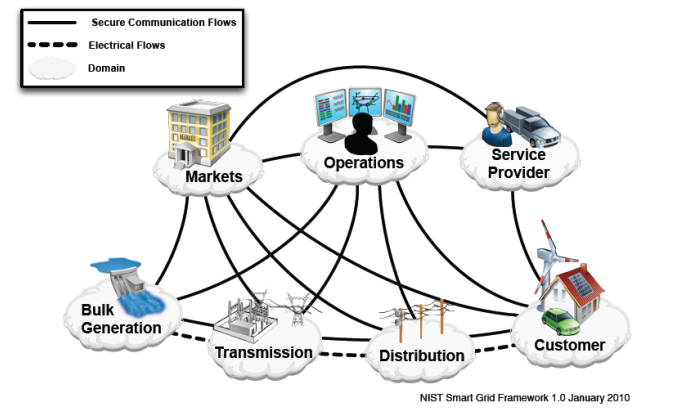
\includegraphics[width=0.75\textwidth]{/Users/rafaelremondes/UM/MEI/Thesis/DistributedAggregationAlgortihmsSM/Writing/Images/NIST_model}
\caption{\label{fig:NIST_model} NIST Conceptual Model for SG}
\end{figure}
Costumers, the end users of electricity, Markets, Service Providers, Electricity Companies, Operations, Managers of the Movement of electricity, Bulk Generation, Generation Centers, Transmission and Distribution of energy. 
In \cite{journals/comsur/FangMXY12} it is provided a more technical approach where the SG is separated into three major subsystems:
\begin{itemize}
\item \textit{Smart infrastructure system} embraces the energy subsystem, information subsystem and communication infrastructure subsystem. The energy subsystem is responsible for advanced electricity generation, delivery and consumption. The information subsystems are responsible for information metering, monitoring and management in the context of the SG. Finally, the communication subsystem is responsible for the communication among the various components and also its connectivity.   
\item \textit{Smart management system} Provides advanced management and control services and functionalities, \cite{journals/comsur/FangMXY12} considers this system the key reason why SG can revolutionize the grid.  Most of the new grid goals are related to energy efficiency improvement, supply and demand balance, emission control etc. and it is the scope of problems the management systems tries to resolve.
\item \textit{Smart protection system} Provides advanced grid reliability analysis, failure protection, security and privacy protection services.
 \end{itemize}
Smart Grids are about improving the current power grid in therms of reliability, energy efficiency and costs  while providing a better and more flexibly service to the costumers. These improvements are made possible with the integration of ICT into the power grid, leading to a opportunity for the dawn of new software applications. In \cite{Andrea} it is stated that Service Oriented Architectures represent the type of software architecture that satisfies the characteristics needed for a SG software: capable of sustaining a set of systems and applications that are diverse, highly distributed and with constrains for security and timing.  In  \cite{Andrea} it is provided an overall picture that show that show the interaction between these type of software and the physical infrastructure.
\begin{figure}[h]
\centering
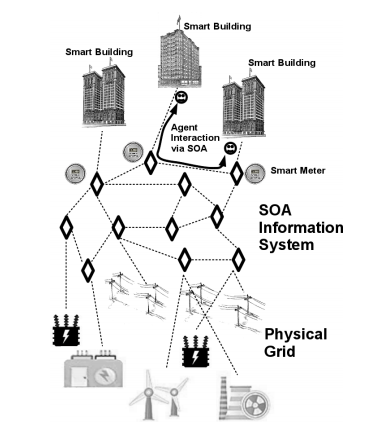
\includegraphics[width=0.75\textwidth]{/Users/rafaelremondes/UM/MEI/Thesis/DistributedAggregationAlgortihmsSM/Writing/Images/interaction}
\caption{\label{fig:Interaction_model} Smart grid physical and information infrastructure}
\end{figure}

\section{Smart Grid Communication}
The most important question regarding the communication is "\textit{ what network and communication should be used}"\cite{journals/comsur/FangMXY12}? Since there is no standard communication system in SG, several communication solutions were proposed divided into wired and wireless communication.\\
Wired solutions are normally more costly to implement than Wireless, mainly because of the need, in some cases, to install or deploy from zero a physical infrastructure like cables to link the components in order to enable communication.  Wireless communication can be a better option in terms of cost, time to deploy and furthermore they are normally more suitable for remote end applications \cite{parikh2010opportunities}. However, they lack of some performance compared to wired solutions, specially in speed. Also, the costs of deploying an wired communication infrastructure can be reduced if they are implemented in the existing infrastructure, case of power line communication that use the power cables.\\
There are several wireless possibilities for communication.\\
\begin{itemize}
  \item \textit{Wireless Mesh Network} (WMN) is a communication network made up for radio nodes organized in a mesh topology\cite{journals/comsur/FangMXY12}. It increases reliability and automatic network connectivity, has large coverage and high data rate.
\item \textit{Cellular Communication Systems}  GSM and 3G. Useful in case of low computation power devices such as the meters. It is quick and low-cost to obtain data communications coverage over a large geographic area \cite{akyol2010survey}. There several solutions that use a Short Message Service communication to send the meters data.
\item \textit{Wireless Communication based on 802.15.4} ZigBee is a wireless communication that is recommended to be used in SG considering the IEEE 802.15.4 protocol stack\cite{parikh2010opportunities}. ZigBee is designed for radio-frequency applications that require low data rate, long battery life, and secure networking. Selected as the communication technology for the smart metering devices\cite{farhangi2010path} because it provides a standardized platform for exchanging data between smart metering devices and appliances located on costumer  premises\cite{journals/comsur/FangMXY12}.  WiMax, WirelessHART and ISA100.11a are other examples of wireless communications based on the IEEE 802.15.4 protocol.
\end{itemize}
Other examples of wireless communication are satellite cognitive radio and  microwave communications.
Fiber-optic Communications and Power-line Communications are some of the wired communication possibilities. Power-line communication has the advantage of being already installed, so the cost of deployment is less expensive than other wired solutions. Fiber-Optic has also the advantage of being fast  but it can be more expensive to deploy because of the need to implement from zero in an infrastructure that lacks cables with that sort of technology.\\



%%%%%SMART METERS-----------------%

\section{Smart Information SubSystem}\label{sec:sginformation}
This part of the SG refers to the whole information that is collected by sensing the consumers consumption and its management . The data collected is often used for billing, grid status monitoring and user appliance control \cite{journals/comsur/FangMXY12}. It is aggregated and collected, afterwards \textit{smart management} is ideally performed on the data.\\
An important concept in the information subsystem  is the \textit{Smart Metering} and the Smart Metering System or Automatic Meter Reading \nom{AMR}{Automatic Meter Reading}. This system is responsible for collect the data from the measurements that are performed by the SMs.\\
Other part of the Smart Information SubSystem is the \textit{Smart Monitoring and Measurement} which can be approached by either \textit{sensors} or \textit{phasor measurement units}(PMU). \textit{Sensors} are used for detecting failures, tower collapses, hotspots and extreme mechanical conditions. They can also provide real-time diagnose of the grid status. PMU's are devices that measure the electrical waves on a electrical grid to determinate the health  of the system. These systems collect information regarding the status of the grid in order to monitor it and detect failures and outages.\\
 The Smart Metering Systems  only collects data from SM's and it only embraces the management of that data.The management refers to the whole information analysis and modeling, integration and optimization.In this specific part of SG there are several areas of research that represent a new set of opportunities.

\subsection{AMR and AMI}\label{subsec:amrami}
As referred in this document, the smart metering system is composed by smart meters that sense the energy consumption and send  their data to a Gateway or a Data Collector. It can also be defined as AMR or  \nom{AMI}{Automated Metering Infrastructure}. In \cite{journals/spm/ErkinTLP13}, the AMR is described in more detailed as an "\textit{technology of automatically collecting diagnostic, consumption and status data from energy metering devices and transferring that data to a database for billing troubleshooting and analyzing}".\\
 The Automated Metering Infrastructure is a more sophisticated version of the traditional AMR, it provides two-way communication, enabling a more sophisticated control of a smart meter behavior. Therefore, all of the meter information is available in real time, allowing improved system operations and  costumer power demand management\cite{journals/spm/ErkinTLP13}.  AMI has also the ability of reconfigure from communication failures, perform outage management and reporting, service connect and disconnect and it also enables time stamping of meter data \cite{hart2008using}. AMI is built upon AMR. \\
Current SM enable two-way communication, an important part of the benefits that come from the usage of this new meters, comes from two-way communication, also two-way communication is not only important for behavior control and outage detection, it enables the realization and implementation of in-network algorithms. Now it is more correct to assume that every AMR has an AMI built upon it enabling two-way communication.\\
In the pilot projects studied, a smart metering system is, of course, composed by the smart meters. The common part is that in a  pre-defined period of time, the devices send the consumption data. In projects, a cloud based service is used for the  SM to send the data . In other cases, substations that work as data collectors are used to concentrate  the consumption information from the SMs connected to it, usually a whole neighborhood, afterwards, the data from the substations is sent to a data center. In small SG, there is no central data center. The substations communicate with each other.\\ 



\subsection{Smart Meters}
Smart meters are devices that sense the energy consumption. They are installed in the costumer side,  households or in  industrial facilities, depending on the costumer nature. Playing a major role in the information subsystem, smart meters present several number of challenges in sensing and analyzing\cite{journals/spm/ErkinTLP13}. SMs, more specifically, the Smart Mettering System has also the denomination of AMR(Automatic Meter Reading). In \cite{khalifa2011survey} the AMR is referred as the technology whose goal is to help collect the meter measurement automatically and possibly send commands to the meters.\\
As referred in the previous section, the main function of a smart meter, and all meters, is sense the consumption in the costumer side. The feature of sending their data, allocate and aggregate the information that comes from many meters allows a company to remotely read the consumers' consumption at each household, without the need to actually go to the premises and without notifying the costumers\cite{Ericsson_2}. Jorge Vasconcelos \cite{RePEc:erp:euirsc:p0193} enlightens in his work the potential benefits of the smart meters, for  example, the potential benefits for customers are customer awareness and energy saving, more accurate meter reading, billing, better service quality, greater tariff variety and flexibility, improved conditions for vulnerable customers, easier comparability of offers and it is easier to change supplier. \cite{khalifa2011survey} states some benefits of the smart metering system: Real time pricing, power quality measurement, automated Billing, Load management,, Remote Connect/Disconnect, Outage notification and Bundling with water and gas.\\
Privacy and security are important concerns when dealing with the sensed information. There are many privacy issues considering that external parties access the consumer energy consumption. Some are authorized parties, but there is a risk of an unauthorized access of this data, leaving to some security and privacy dangers. For example, by analyzing the data, one could determinate which devices are plugged in at some specific time, giving for example information about if there is people in home or note. Many pieces of work propose solution to securely store this sensible information. Although privacy and security are out of the scope of this work, it is important to mention this point.\\

\subsection{Smart Grid Projects}
So far there aren't standards to realize the Smart Grid, as it was aforementioned, not even a complete and specific definition about what is a Smart Grid. Even without a specific definition regarding the standard model and communication, there  are common concepts that are well accepted and visions that are transversal . The introduction of communication and information technology into the grid, the idea of a consumer that is not only a consumer but also a small producer that can supply the grid and itself with electrical energy, the remote control of the components like electrical cable and station and more, are ideas that seem to be features that all future SG will have. In order to understand how it is currently the status of the SG and the directions it will take in the future, we analyze several pilot projects and companies that are know a days trying to implement the new grid.
\subsubsection{Opower 4}
Opower\cite{website:opower} iis a company that promises to help costumers to reduce their energy consumption. They provide a cloud based service to gather data regarding the costumers information about their energy consumption, and using big data and behavioral science they provide reports to the costumer with their consumption history in the time period that report is about. Also, the reports give tips and advices where the consumer can reduce the energy consumption, and therefore, reduce the energy bill.\\
One of the version of the promised platform, one of the most recent, is called Opower 4. Opower 4 works as a service platform, is a \textit{Software as a Service} platform. The model is like the general model for the SG Information subsystem described in section \ref{chap:sg}. Households using this services have a smart meter installed, every 15 minutes, the device send the data to a cloud through a cloud based service. The collection of the data is only made in one point, in a Data Center that concentrates all data. There is no reference regarding the number of data centers that the company uses. Big Data is performed in the data. Mainly, as it was stated, the platform exists for billing proposes and to raise awareness in the costumers so that they reduce their consumption with reports that have statistics of each household. For example, one costumer comparison with the neighborhood and what devices are consuming more or less.
\subsection{DEHEMS Project}
The DEHEMS project \cite{website:dehems}t is an infrastructure that reasons about the household's energy behavior and tests various persuasive techniques effectiveness. The system receives energy information from several sensing devices, including the ones that sense electrical consumption. The special feature about the DEHEMS project is that it uses Informix TimeSeries \cite{website:informix} that is a built­in feature of Informix, a database type of IBM, that adds support for managing time series (time­stamped) data, this feature is specially important in the management of data regarding the reading of the meter.\\
This project operates in the distribution grid. The model also includes de household, where several sensors are installed, not only for electricity, but also for gas and water. Each sensor, with a 433Mhz Radio, takes reading every 6 seconds and sends it to a DEHEMS Gateway that aggregates all the information about the house. The data of all the Gateways is concentrated in a Informix database so that big data operations can be performed on it.\\The goal of this project is the same as the aforementioned project, raise awareness in the costumers by generating statistics abou each household consumption(CO2 emissions, cost of the energy, history of consumption and comparison with the other consumers) and send it to the consumer.
\subsubsection{Pecan Street Project}
The Pecan Street Project\cite{website:pecan} is a research project / is researching a project?? in Smart Grids by Pecan Street Inc., a University of Texas­based research organization. Started in Austin an then expanded to other cities and states. The focus of the research is mainly in the information subsystem of Smart Grid. One of the project goals is to understand how to lower the carbon emissions by learning how energy is being used among homes. But understanding the “how†is only half of the challenge: Pecan Street also seeks to understand what homeowners need in order to manage their energy use.\\
As the other, it operates in the distribution grid and it works in a similar way as the DEHEMS project. In each house, there are several sensors installed to sense the consumption in each device, for example the Air Condition System. The sensors send their data every 2 seconds to the gateway and then to the smart meter every 15s, the meter sends the collected information from the gateway to a data center every 15 minutes. In the gateway it is performed an estimated average of all devices connected to a sensor. The consumption data is in the end used for statistical analysis to produce results about the consumer energy consumption. With this information, the Pecan Street Project staff pretends to lead their costumers to use their energy more efficiently.
\subsubsection{Smart Meter Data Stream in the Cloud}
This is a solution proposed to handle the SM data in a distribution electrical grid which is in
\cite{lohrmann2011processing} for real time pricing. The simulation considers a set of 1 million meters connect via TCP/IP to a data center/Cloud. Every second, each SM sends a package containing information about the electrical consumption of an household. The cloud model is composed by layers. Since every moment a new package arrives, it is like a stream, so several stream tasks are created in the lowest layer to handle the incoming data. In the upper level, within the cloud, aggregation tasks are created and they work in parallel to handle the information that comes from the lower level, the stream tasks. As the traffic increases or decreases, more aggregation tasks are created or deleted accordingly. In the paper simulation, 2 aggregation task were created. In the highest lawyer there is one real time pricing task that has the role of updating the energy price according to the amount of the energy consumed.\\
This paper offers a solution to handle smart meters data to provide a real­time pricing policy to balance the
demand of energy and also to continuously monitoring of the meter, mainly to prevent outages and blackouts during peak time.
\subsubsection{Inovgrid/InovCity}Inovgrid\cite{matos2013inovgrid} is a project powered by EDP, Energias de Portugal, that pretends to modernize the portuguese electrical grid, more specifically, the distribution grid, in other words, the project aims to transform the traditional grid into a smart grid by adding information and communication technology. This is still a pilot project, there is no mass scale attempts yet to fully implement.So far, there is only a pilot project called the InovCity in the city of Évora that consists of a smart grid small experiment, with the installation of several smart meters and sensors in some of Évora households. \\
In further detail, the InovCity model can be explained by dividing the grid into three smaller networks: a Home Area Network(HAN), a network in each house, whereas each device has a sensor that communicates with the smart meter installed in the house. In the set of devices that composes the HAN, electrical vehicles are also included.
Local Area Network, a set of households, a neighborhood connect to a DTC/substation that communicates through the electrical cables, PLC Prime and LMS protocol. Finally, the wide area network that embraces all the other minor networks\\
In terms of number, in InovCity 300 000 Smart Meters and 300 DTC/Substations were installed. The Smart Meteres communicate the consumption of an household every 15 minutes to a Substation which therefore communicates to other substation and finally to a central facility. Each substation has the capability of performing data analysis and process data function, so, depending on the type of analysis, the substation can perform it locally. Basically, the whole collection of data works in an hierarchical way, the data is collected in every smart meter regarding the information about every device with a sensor, a substation aggregates information about the houses connected to it, the upper level of substation collects the information of the other substation connected to it in lower levels, and finally the central facility concentrates all, working as a "sink".\\
There are 3 goals the company claims to achieve with the InovCity architecture. More energy efficiency by raising awareness in the clients with detailed information about their consumption. Increase Operations efficiency and reduce its costs by remotely perform any needed operations from a central station instead of doing it locally. Finally, commercial benefits by having a real time consumption instead of an estimated one and more accurate control by having a real time alarm of a failure in a SM..
\subsubsection{PowerMatching City}
PowerMatching city\cite{website:powermatching} is a pilot project of a self sustainable micro smart grid
implemented and tested in Hoogkrek, a town in the north of Netherlands. Opposite to the other examples, in this case there were grid in considerable size and they were more focused on reducing the consumption and improving the performance of the grid, in this case, the goal is to create a self­sustainable city when it comes to energy consumption. In this city, the costumers can buy and sell their energy. They buy it from a market that is composed by small producers in the city that can generate energy through renewable sources, and, therefore, they can sell it too. This way, the city becomes independent from major electrical companies. \\
In PowerMatching, each household has a smart meter that has the information about the consumption of each device and also about the energy produced. The information is sent by the smart meter to a coordinator/data collector through an VPN communication infrastructure. Also, an ADSL communication channel is used between the coordinator and the houses connected to it to prevent the occurrence of faults. The coordinator is responsible for collecting the information about the energy consumed and produced, and generating the prices accordingly, working as a market. This idea can scale adding more coordinators that are connected and communicate among each other to work as a whole market.\\
In the implementation in Hoogkrek, 25 Household had an SM installed to the PowerMatching city network with, at least, one collector/coordinator. Data is collected in every coordinator station, therefore, the process in the
station works in a lawyered process, the lower levels receive and collect the information, send it to the upper level in  the bif format, to buy or to sell energy that are communicated to every house connected. It is not
mentioned what is the interval by which the prices of the energy are changed, but we can admit that it is not about the time, but in terms of supply and demand as in all markets.\\
Also, the system contemplates three web portals for data: user Portal where the user can check her/his stats about energy consumption/production, operator Portal which is mainly used for operations(monitoring and detecting failures, data analysis that generates reports used mainly for research proposers and for the development of the project.\\
The main goal is to organize a market whereas all community is independent from global companies. The measured data is used and aggregated mainly for price proposes, i.e., following the market rules, the data is used to give selling and buying prices. Also, in terms of singular house, the data is used also by the system to buy or sell the energy. If a house has low energy supply plus high demand, the systems should buy it, on the other hand, if there is a surplus, ideally it should be sold it to the market.\\
\\
There is other examples of other smaller SG models that represents more and idea. Keita Suzuki \textit{et al} \cite{DBLP:conf/isgteurope/SuzukiNYKMKA13}  presents a particular case in a office building in Japan(Heating ventilation and air conditioning facilitie,HVAC) where existis the need to aggregate power curtailments from hundred or thousands of distributed HVAC facilities. Several smart meters where placed, connected to a Gateway that receives the consumption data for daily or monthly billing.  The Gateways are connected to a central ADR, Aggregation Cloud, which aggregates all the consumption.\\
Another work using a \textit{de-centralized} way is in Rottondi \textit{et al}\cite{rottondi2012}.  The smart meters generate the energy consumption measurements, the Gateways securely aggregate the metering data and external parties access the aggregation results. Each meter is directly connected to a Gateway, receiving data from a limited number of meters. At regular time intervals, 15 min in this case, the meter generate a measurement and send it to the Gateway.















 %
\chapter{Wireless Sensor Networks}\label{chap:wsn}
Wireless Sensor Networks(WSN) are \textit{ad-hoc} networks composed by tiny devices with limited computation and energy capacities. These tiny devices, sensors, are so called tiny because of their low capability of computation, communication and storage. The WSN  low-cost sensors monitor physically on environmental conditions, such as temperature, sound, vibration, pressure, monitor pollutants and to cooperatively pass their data through the network to a main location(sink node) via multi-hop wireless links\cite{asad2013survey} or to their peers.\\ 
WSNs act under severe technological constraints: individual sensors have severely limited computation, communication and power(battery) resources and need to operate in settings with great spatial and temporal variability.The ad-hoc nature of a WSN implies that sensors are also used in the network infrastructure, i.e., not just sending their own data and receiving direct instructions but also forwarding data for other sensors. Modern networks are bi-directional, enabling control of sensor activity but some WSN could not have bi-direccional communicatin  due to low computation power of the sensors. The development of wireless sensor networks was motivated by military applications such as battlefield surveillance.\\
Today, WSN networks are used in many industrial and consumer applications like industrial process monitoring and control, machine health monitoring and so on. Some of WSNs requirements are:  large number os nodes, low energy use, network self organization, collaborative signal processing and querying ability.\\
 WSNs are becoming increasingly popular in many spheres of life \cite{castelluccia2005efficient}, they also have the capability of forming the sensor web services which can be considered as an extension of the future internet towards smart devices, Internet of Things(IoT)\cite{asad2013survey}.  \\


\section{WSN and  The Smart Grid}
Considering the overall appliances, WSNs has also several applications in the SG. Furthermore, the AMR could be considered as a specific example regarding the appliance of WSN. It can be implemented the proposed WSN solutions for data aggregation in AMR .\\
Recently, WSN has been widely  recognized as a vital component of the electric power system\cite{journals/ijdsn/Liu12}. WSN contains a large number of low cost and multifuncional sensor nodes which "\textit{can be of benefit to electric system automation application, especially in urban areas}"\cite{RePEc:eee:rensus:v:15:y:2011:i:6:p:2736-2742}. The collaborative and context-awareness nature of WSN brings several advantages over traditional sensing include great fault tolerance, improved accuracy, larger coverage area and extraction of localized features \cite{journals/ijdsn/Liu12}. Sensor nodes can monitor the overall network.\\
WSN could apply to several features in the SG: basis measurement, smart voltage sensors, smart capacitor control, smart sensors for outage detections, smart sensors for transformer monitoring, high voltage line temperature and weather condition sensors, distributed generation, smart gird storage and, referenced before and more importantly for this work, WSN for AMI( Advanced Metering Infrastructure) or AMR.
A specific example is in \cite{journals/ijdsn/Liu12} where a WSN could apply perfectly to a household or House Area Network(HAN) . In section \ref{sec:Smart Grid Communication} it is mentioned ZigBee as communication technology in Smart Grids. Due to its reliable wide area coverage and predictable latencies, ZigBee is a suitable choice for a Local Area Network such as a household or a neighborhood. As a example in \cite{journals/ijdsn/Liu12}, a WAMR(Wireless Automatic Meter Reading) can determinate real-time energy consumption of the customers by sensing each device that have a wireless sensor on it. The smart meter within the household perform an interface that translates, summarizes and aggregates data of power usage and presents it to the power utility.\\ 
Other examples of WSN appliances in SG are founded in \cite{journals/ijdsn/Liu12}. WSN could apply in Power Delivery and in Power Generation as well since the sensors can monitor the deliver systems, in the first case, and monitor the energy generated in the second case.\\
Although very similar, there are some differences between WSN and Automatic Meter reading. Such diferences are stated in \cite{khalifa2011survey}. For example, individual measurments must preserve its informations. In WSN, sink doesn't care about inidivudal data but in AMR, aggregation nodes must preserve the unique measurments, plus, the meters must have a unique indetifier that links the smar meter to a household/costumer/producer. Other  important difference is the fact that AMR must support bi-direccional communications, some of WSN only have one way communicaton. Futhermore, Smart meters have fixed positions on contrary to some WSN, base stations may need to disconnect/connect to a specific costumer. Even in security, there are some differences. The main security concern in WSN is to preserve the privacy of data, in SM, altough privacy is an important issue, integrety of data is the main concern.\\
WSN, even considering the diferences to AMR, it provides a variety of solutions and gives some insight to understand and comprehend the problem of distributed aggregation in AMR since WSN is a well studied subject.The topology we can find in some WSN can apply to the ones in the AMR. So, even with differents communication infrastrutures or different computation powers,  from the topological view, both networks are very similar.\\

%
\chapter{Distributed Data Aggregation}
\section{Definition}
Data aggregation is a technique that consists, on its basis, in reduce the amount of data collected, reducing the resources needed to process it.  According to \cite{journals/corr/abs-1110-0725}, data aggregation is  considered a subset of information fusion, that aims at reducing the handled data volume. A more precise definition is given in the same report:
\begin{definition} An aggregation function $f$ takes a multiset of elements from a domain $I$ and produces an output of a domain $O$.
\begin{equation*} f : \mathbb{N}^I \to O \end{equation*}
\end{definition}
The order in which the elements are aggregated is irrelevant and a given value may occur several times. As the main goal of data aggregation, the aggregation function aims to summarize information. The result of an aggregation takes less space than the inputed multiset (element from $\mathbb{N}^I$).\\
Distributed data Aggregation or \textit{in-network} aggregation means that it is a task which is distributed among several nodes in the network. In contrary of a \textit{centralized} arquitecture, where a central node compute all the data and performs the aggregation function, a \textit{de-centralized} aggregation distribute the data, hence the effort to compute the aggregation function is reduced.
\subsection {Decomposable functions}
\todo{Correct definition? Need to specify more why decomposable functions could be computed in a parallel or distributed way}
For some aggregation function, one node may need to perform a single computation operation involving all the elements of the multiset, requiring more resources than the ideal ones. So, in order the distributed the effort to compute the multiset, there are some aggregation function that are decomposable. Meaning that, the effort could be done in a distributed way. A definition for decomposable function is also given in \cite{journals/corr/abs-1110-0725}:
\begin{definition} An aggregation function $ f : \mathbb{N}^I \to O$ is said to be self decomposable if, for some (merge) operator $\diamond$ and all non empty multisets $X$ and $Y$:
\begin{equation*}f(X \uplus Y) = f(X) \diamond f(Y) \end{equation*}
\end{definition}
The $\uplus$ denotates the standard multiset sum. The operator $\diamond$ is commutative and associative \cite{journals/corr/abs-1110-0725}. Some functions that are self-decomposable:
\begin{align*}SUM ({x}) &= x,\\
SUM(X \uplus Y) &= SUM(X)+SUM(Y).\end{align*}
\begin{align*}COUNT ({x}) &= x,  \\
COUNT(X \uplus Y)& = COUNT(X)+COUNT(Y).\end{align*}
\begin{align*}MIN ({x}) &= x,\\
MIN(X \uplus Y) &= MIN(X) \sqcap SUM(Y).\end{align*}
\begin{definition}
An aggregation function $ f : \mathbb{N}^I \to O$ is said said to be decomposable if for some function $g$ and a sel-decomposable aggregation function $h$, it can be expressed as:
\begin{equation*}f=g \circ h\end{equation*}
\end{definition}
As the definition above, stated in \cite{journals/corr/abs-1110-0725}, self decomposable functions are a subset of the decomposable functions. One example of a decomposable functions $AVERAGE$:
\begin{align*} 
AVERAGE(X) &= g(h(X)),\\
h({x}) &= (x,1),\\
h(X \uplus Y) &= h(X) + h(Y),\\
g((s,c)) &= s/c. \end{align*}
Another example is the $RANGE$ which gives the difference between the maximum and minimum value.


\subsection {Duplicate sensitiveness and idempotence} 
For some functions, the presence of duplicate results does not affect the result. Examples of this aggregation functions are $MAX$ and $MIN$, where the result on only depend on its \textit{support} set(obtained by removing all duplicates)\cite{journals/corr/abs-1110-0725}. Others, like $SUM$ or $COUNT$, the duplicate numbers are relevant. This propriety is called duplicate sensitiveness, it is relevante in distributed aggregation. Using an idempotent binary operator on the elements of the multiset helps obtaining fault tolerance \cite{journals/corr/abs-1110-0725}.
\begin{definition}
An aggregation function $f$ is said to be duplicate insensitive if for all multiset $M, f(M) = f(S)$, where $S$ is the support set of $M$.
\end{definition}
A taxonomy table of aggregation is in \cite{journals/corr/abs-1110-0725} and it is presented below.
\begin{center}    
\begin{tabular}{|c||c|c|c|}
    \hline
                                         &   \multicolumn{2} {|  c  |}{ Decomposable}                                               &    Non-decomposable \\ \hline
                                         &    Self-Decomposable      &                               &  \\ \hline
      Duplicate insensitive  &    $MIN,MAX$                  &     $RANGE$         &  $DISTINCT,COUNT$ \\ \hline
      Duplicate sensitive     &    $SUM,COUNT$           &     $AVERAGE$     &  $MEDIAN,MODE$ \\ \hline
    
    \end{tabular}
\label{Taxonomy of aggregation functions}
\end{center}

\section{Distributed Data Aggregation Algorithms}
\todo{Review DDA, Write the algorithms or just the type?}
In \cite{journals/corr/abs-1110-0725} is also presented a simple taxonomy of the existing algorithms that performe distributed data aggregation. First it is analyzed the algorithms from the communication prespective, i. e., the routing protocols and the intrisic topologies, afterwards, it is analyzed the computation issues, how the aggregation functions are computed by the algortihms.


\subsection{Communication}

\subsubsection{Hierarchy-based approaches} 
Traditionally, existing aggregation algorithms operate on a hierarchy-based communication scheme. This is \textit{structed} communication scheme. It is required to know in advance the topology of the network. A hierarchy communication tree is constructed, with several levels of nodes. In the root of the tree is a main repository of all data, denominated as sink. Besides the sink, other special nodes can be defined to compute intermediate aggregates, working as aggregation points that forwards their results to upper level nodes. There are generally two main phases, \textit{request} phase, corresponding to an aggregation request spreading through all the nodes, an the \textit{response} phase where all the nodes respond to the request sending their aggregation results. Some specific examples of these kind of communication are presented.\\
\\
\textbf{\textit{TAG}} The tiny AGregation algorithm that suits for ad-hoc networks described in \cite{madden2002tag}. This algrotihm requires the previous creation of a tree-based routing topology, and the continous maintenance of such routing structure in order to operate over mobile networks. TAG provides a SQL-like declarative language to the users. The algortihms consists of two main phases, the \textit{distribution} phase, i which a aggregation query is disseminated through all the spanning tree, and a \textit{collection} phase, where the values are aggregated. A waiting time is required to conclude this two phases.\\
\\ 
\textbf{\textit{DAG}} An aggregation scheme fro WSN is proposed in \cite{motegi2006dag} that aims to reduce the number of message losses. \todo{resume this shitty algorithm}\\
\\
\textbf{\textit{Sketches}} Algorithm proposed in \cite{considine2004approximate} that uses smal sketches. Based on the probabilistic counting sketches technique that estimates the number of distinct elements in a data collection. Like other algortihms of this type, is uses two phases: the sink propagates the aggregation request accross the network and then the results are collected back to the sick. In the first phase, all nodes compute theirs distances to the root, in the sencod phase the partial aggregates are computed across the routing structure, using the adapted counting sketch scheme, and send to the upper levels in sucessive rounds.\\
\\
\textbf{\textit{I-LEAG}} Cluster-based aggregation approach designated as I-LEAG is in \cite{birk2006veracity}. The routing structure of this algortihm is composed by a hierarchy of clusters or partitions. A single pivot is desginated for each cluster and the root is the pivot of the upper level cluster. This structure can be consider similar as we can see in networks with \textit{super-peers}, but organized in a tree structure. The algorithm works as follows: each cluster check local conflicts that are reported to the pivot, then the pivot computes the new aggregate and multicast the result, each node must forward the received result to the nodes outside the cluster.\\
\\
\textbf{\textit{Tributary-Delta}} 
This approach mixes the tradional use of tree and multi-path routing schemes, dividing the network in two routing regions: \textit{delta}(multipah) and \textit{tributary}(tree). Use tributaries in regions with low rate of message losses to take advantage of tradiontal tree schemes and delta in regions with higher rate of message losses(mostly regions near the sink with the aggregate of several nodes).
\todo{resume other approachs}
\todo{Ring Based Approachs, Flooding and Randomized necessary or relevant?, IDEA: state the hierarchy and gossip approach and then the hybrid aproach combining the two}

\subsubsection{Gossip-based approaches}
This type of approach is reffered as an \textit{unstructed} approach, contrary of a aforementioned \textit{structed} approachs. In this type of scheme there is no previous knowledge of the topology of the network or any specific structure. The information or messages are commonly disseminated accross the network without follwing any specifc topology, the informartion it is passed node to node, or nodes, like a infectious disease or a gossip,i.e., a "infected" node sends a message to a random subset of nodes. This type scheme tend to allow a robust(fault tolerant) and scalable information dissemenation over all the network\cite{journals/corr/abs-1110-0725}\\
\\
\textbf{\textit{Push-Sum Protocol}}  Push-sum protocoI\cite{kempe2003gossip} is a gossip-based protocol to compute aggregation functions. Along discrete times $t$, each node $i$ maintains and propagates information of a pair of values $(s_ti,w_ti)$ where $s$ represents the sum of the exchanged values and $w$ the weight associated. In each iteration, a neighbor is choosen uniformly at random and half of the actual values are sent to the target node and the other hald to the node itself. Upon reveived, the local values are updated, adding each value from a received pair to its local component\cite{journals/corr/abs-1110-0725}.\todo{review this definition, too much alike}

\subsubsection{Hybrid approaches} 
Hybrid approaches propose a solution that merge both hierarchic and gossip-based approachs, using the high accuracy and efficiency of the hierarchic based schemes and the robustness of the gossip approachs. In the disadvantages of one approach , the other one has it as an advantage, Hybrid approachs aim to merge the advantages of both schemes to elimanate both disadvantages.\\
\\
\textbf{\textit{Chitnis et al, 2008}} Chitnis et al.\cite{chitnis2008aggregation} proposed an hybrid approach, using TAG as an hierarchy-based approach and Push-Sum as a gossip-based protocol. This hybrid approach divides the network node in groups. Inside each group, a gossip-based protocol is used. In each group, a leader is elected to further performe a hierachic communication with other  leaders nodes regarding the aggregation results from the gossip group. 

\subsection{Computation}
\subsubsection{Hierarchical}
The input is separted into groups so it can be computed in a distributed hirarchical way.  Depends on the previous formation of a communication structure such as tree or cluster. Some node work as \textit{forwarders}, just forward data to upper levels of the hierarchy, and others work as \textit{aggregators}, apply the aggregation function directly to all received input and then work as a normal \textit{forward} node. This class of algorithms allow any decomposable function with high accuracy without the presence of faults. Algortithms of this class were aforementioned.
\subsubsection{Averaging}
This class of computation scheme is based on a iterative computation of partial aggregates, where all nodes share their results among the network and all of them contribute for the final result. This scheme provides high accuracy, considering that all nodes converge to the same result. One example of algorithms of this class, are the ones with gossip base communication scheme, since the results of the aggregates could be share randomnly with the neighbor nodes. Due to its nature, Averaging algorithms tend to by highly robust, i.e., tolerant to faults on opposite of the structed algrotihms. Decomposable and duplciate sensitece functions can be be computed in this class.\\
\todo{specify the mass conservation concept?}\\
\textbf{\textit{Push-Pull Gossiping}} Similar to the aforementioned \textit{push-sum protocol}, the push-pull gossiping\cite{jelasity2004epidemic} performes an averaging process. This algortihm executes an epidemic protocol to perform a pari-wise exchange of aggregated values between neighbor nodes\cite{journals/corr/abs-1110-0725}. In periodic intervals of time, a node send its value to a randomly selected node and waits to receive a result back, the response from the selected node. Afterwards, an average with the new value and the present value its perfomed in order to calculate and store a new one. When a node receives a value from another node, the same process is performed, send the current value and calculate a new one from the average of the received value and the current one.\\ 
\\
\textbf{\textit{DRG(Distributed Random Grouping)}} This approach \cite{chen2006robust} randomly creates groups across the network in which aggregates are sucessfully computed. There are three modes a node can performe:\textit{leader,idle} and \textit{member} which corresponds to three phases. First every node is in \textit{idle} mode, them every node broadcasts a Group Call Message, pretending to be a group leader(with a pre-defined probability associated ) and waits for members. The nodes who receives the group call, respondes to the first one received with a JACK(Joining Acknowledgment) tagged with their aggregated value becoming a member of the group. Finally, the \textit{leader} gather all the aggregated values, computing the aggregation function($AVERAGE$) and broadcasts a Group Assignment Message with the  final result. Every group member waits unit it receives the result from the leader to update its local value and them returns to  \textit{idle} mode.\\
\\
\textbf{\textit{Flow Updating}}\todo{finish this shitty algorithm}\\

\subsubsection{Sketches}
Algrorithms based on the use of an auxilary data structure with a fixed size that holds a \textit{sketch} of all network values. Input values are used to create \textit{sketches} that aggregated across the network, using specific operations to update and merge them. The agregation could be done using multiple paths. This type of algorithms enable operations of order and duplicate insentitive. The computational cost of this class depends mainly on the resources used to produce the result by the estimator and the complexity of the operations to produce the \textit{sketches}. This kind of algorirthms tend to be very fast, depending on the dissemination protocol used to propagate the sketches, but lack accuracy because they are based on probabilistic methods.\\
\\
\textbf{\textit{RIA-LC/DC}} Algorithm proposed in \cite{fan2008efficient}, a multi-path routing aggregation approach. The algrotihm consists of two phases. First a aggregation request is sent by the sink throughour the whole network, creating a multipath routinh hierarchy. Second, starting in the lower leves, each node generates a \textit{sketch} correspondent to its current state and sent it to the nodes in the upper level. The node that receives the \textit{sketch}, creates a new one combining tis current value and the received \textit{sketch} and send it to the upper node until the top is reached where the sink computes the aggregation estimate.
\\
\textbf{\textit{Extrema propagation}}
This approach redices the computation of an aggregation function\cite{journals/corr/abs-1110-0725}. A vector $x_i$ of $k$ random number is created at each network node $i$. Random numbers are generated according to a known random distribution, using the node initial value as an input parameter. The execution of the algorithm consists os the computation of the pointwise minimum between all exchagend vectors. At each node, the obtaind vector is used as a sample to produce an aproximation of the aggregation result. This algorithm is focused ob obtaining a fast estimate, tather than an accurate one. 
\subsubsection{Digests}
This class of algrotihms allow the computation of more complex functions like meadian or mode than the normal aggregation function such as $SUM$ or $AVERAGE$. This algrotihms produces a \textit{digest}, data structure with a bounded size that holds an aproximation of the statistical dristribution of input values in the whole network, that summarizes the system data distribution, an histogram. The accuracy of this calss of algortihms depends mostly on the quality and size of the obtained \textit{digest}. Usually requires more resources.\\
\\
\textbf{\textit{Q-Digest}} This aggregation scheme allows the approximation of complex aggregation function in WSN is proposed in \cite{shrivastava2004medians}. Uses an hierarchical routing topology to build and disseminate quantile digests. Each node maintains a quantile digest of the data avilabe, which are built in a botton-up fashion by merging received digest from lower nodes(children nodes). This new quantile digests are compressed according to a specific compression factor. Aggregation functions are computed by manipulating and traversing the quantile structure acording to a specific criteria.\\
\\
\textbf{\textit{Equi-Depth}} Gossip-based approach described in  \cite{horowitz2003estimating}. The scheme executes a  gossip protocol and merge specific function on the exchanged data. Each node keeps a list of $k$ value or \textit{digests}, initially set to its input value. Each node randomly chooses a neighbor to exchange the digest to merge with its own. This round is executed several number of times, producing an aproximation of the network distribution of values. There are four merging techniques \textit{swap, concise, equi-with histograms} and \textit{equi-depth histograms} that are detailed in \cite{journals/corr/abs-1110-0725}.
\textbf{\textit{Adam2}}
Adam2 is a gossip based algorithm to estimate the statistical distribution of values across a decentralized system\cite{sacha2010adam2}. Each node can decide to start an instance of Adam2 where each instance is uniquely identified by its starting node. The statrting node $i$ initializes the interpolation set $H_i$(composed of $k$ pairs of values $(x_k,f_k)$ where $x_k$ represents an interpolation point and $f_k$ the fraction of nodes with value less or equal to $x_k$). The interpolation is initialized by seting $f_k$ to 1 if the node attribute reading $v_i$ is less or equal than the corresponding interpolation value $x_k$, 0 otherwise. Node store a set of interpolaton points for each running algorithm instance.  A new node that learning about the new instance performes a initializtaion ant then starts participating in the protocol. The sets are exchanged like push-pull, the sets are merged by averaging the fraction at each interpolaiton poin. After a predefined number round the CDF is approximated by interpolating the point of the resulting set.



\section{WSN Data Aggregation}
Distributed Data Aggregation in WSN is an widely study subject, with several works and proposed solutions. Distributed aggregation adquires a special importance in WSN, since the sensor are low resources devices so the effort distribution is quite mandatory. The aggregation techniques reduce the amount of data communicated within a WSN and thus conserve battery power \cite{castelluccia2005efficient}.Periodically, as measurements are recorded by individual sensors, they are been collected and processed to produce data representative of the entire WSN.  An natural approach is consider that the sensor send the measured data to special sensor nodes, i.e., aggregator nodes \cite{castelluccia2005efficient}. In \textit{in-network} aggregation nodes forward the aggregated data to a sink that store it.\\
\begin{figure}[h]
\centering
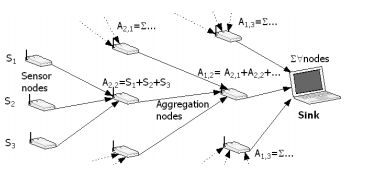
\includegraphics[width=0.5\textwidth]{/Users/rafaelremondes/UM/MEI/Thesis/DistributedAggregationAlgortihmsSM/Writing/Images/INA}
\caption{\label{fig:INAaggregation} Principle of in-network aggregation}
\end{figure}
An example of \text{in-network} aggregation in WSN is in  \cite{castelluccia2005efficient}. In this model, it is assumed that all nodes ate potential aggregators and that data gets aggregated as they propagate towards the sink. The aggregation is set as must being simple not involve any expensive or complex computation. The aggregation requires all sensors to send their data to the sink within the same sampling period so there is a need for a global so that all node can synchronize. Another study is in \cite{Girao2004c}, where a special kind of distributed aggregation is proposed, \textit{Concealed Data Aggregation}. This type of aggregation is defined as an approach than promises the combination os end-to-end security and \textit{in-network} aggregation. In \cite{chan2006secure} it is assumed a general multi-hop network with a set $S={s_1....s_n}$ of $n$ sensor nodes anda a single base station $R$. The aggregation is performed over an \textit{aggregation tree} which is the directed tree formed by the union of all the paths from the sensors nodes to the base station. Another WSN distributed aggregation scenario is presented in \cite{yu2009distributed}. The network model consist of a $n$ sensor nodes and one base station that is also called a sink. Each sensor node can send or receive data to or from all directions. It is assumed that all nodes have the same transmission range for simplicity. A node can either receive or send data at a time and it can receive a data packet correctly when it hears only this packet at that moment.


\section{Smart Metering Aggregation Model} 
There are two main architectures for smart metering considering data aggregation  are \textit{centralized} and \textit{distributed} or \textit{ decentralized}\cite{journals/spm/ErkinTLP13}. In \textit{centralized} fashion, the meters just sense the data, afterwards, it is sent to a central aggregator with higher computation power that holds a central database. In a \textit{decentralized} way, the aggregation role is distributed among several meters, not all of then. This type of aggregation is also called  \textit{in-network} aggregation \cite{Girao2004c}\cite{Castelluccia05efficientaggregation}. The aggregation node in this scheme communicate the calculated energy consumed to an appropriate party such as a energy producer. Typically, this communication occurs once per billable period \cite{journals/spm/ErkinTLP13}. As introduced before, the architecture chosen for this work is \textit{de-centralized} due to the nature of the aggregation algorithms.\\
In the literature, it is possible to find some particular studies. Keita Suzuki \textit{et al} \cite{DBLP:conf/isgteurope/SuzukiNYKMKA13}  presents a particular case in a office building in Japan(Heating ventilation and air conditioning facilitie,HVAC) where existis the need to aggregate power curtailments from hundred or thousands of distributed HVAC facilities. Several smart meters where placed, connected to a Gateway that receives the consumption data for daily or monthly billing.  The Gateways are connected to a central ADR, Aggregation Cloud, which aggregates all the consumption.\\
Another work using a \textit{de-centralized} way is in Rottondi \textit{et al}\cite{rottondi2012}.  The smart meters generate the energy consumption measurements, the Gateways securely aggregate the metering data and external parties access the aggregation results. Each meter is directly connected to a Gateway, receiving data from a limited number of meters. At regular time intervals, 15 min in this case, the meter generate a measurement and send it to the Gateway. The overall scheme is presented in \ref{fig:meterArchitecture}.
\begin{figure}[h]
\centering
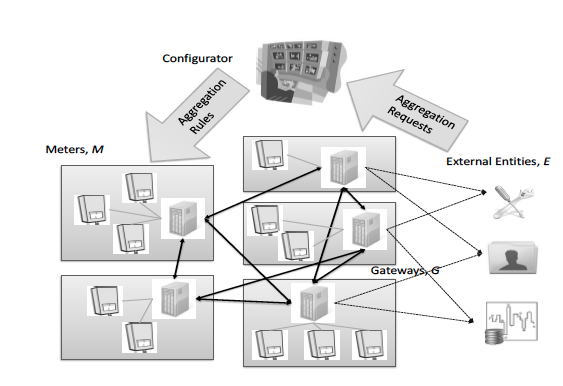
\includegraphics[width=0.5\textwidth]{/Users/rafaelremondes/UM/MEI/Thesis/DistributedAggregationAlgortihmsSM/Writing/Images/meterExample}
\caption{\label{fig:meterArchitecture} The functional nodes of the architecture}
\end{figure}

%
\chapter{Conclusion}\label{c:conc}
%Lá chegará o dia em que haverá algo para concluir.
Until now, much of the work done focused on the analysis of the state of the art in Smart Grids, AMR and in-network aggregation in both AMR and WSN and also the various existing algorithms.

After the state of the art complete, the next phase will be analyze in further detail the selected in-network aggregation algorithm. This analysis will require implementation in simple topologies in order to gain more insight about them. A performance analysis may take place in order to reduce the number of algorithms to be implemented in a SG or AMR topology. Afterwards a selection of a AMR topology will take place. Considering the existing pilot projects, the future topology may be as close to real implementations as possible. The next phase will be implement the algorithms and collect the results. Some improvements to the algorithms should occur so that a better performance may be achieved and aso the better results to the overall grid. 


 % 

%\input{Chapters/Chapter4} % 

%\input{Chapters/Chapter5} % 

%\input{Chapters/Chapter6} % Results and Discussion

%\input{Chapters/Chapter7} % Conclusion

%% ---------------------------------------------------------------------------
% Now begin the Appendices, including them as separate files

% Add a gap in the Contents, for aesthetics
\addtocontents{toc}{\vspace{2em}}

% Cue to tell LaTeX that the following 'chapters' are Appendices
\appendix

%\chapter{Aggregation Functions}
\subsection {Decomposable functions}
For some aggregation function, one node may need to perform a single computation operation involving all the elements of the multiset, requiring more resources than the ideal ones. So, in order the distributed the effort to compute the multiset, there are some aggregation function that are decomposable. Meaning that, the effort could be done in a distributed way. A definition for decomposable function is also given in \cite{journals/corr/abs-1110-0725}:
\begin{definition} An aggregation function $ f : \mathbb{N}^I \to O$ is said to be self decomposable if, for some (merge) operator $\diamond$ and all non empty multisets $X$ and $Y$:
\begin{equation*}f(X \uplus Y) = f(X) \diamond f(Y) \end{equation*}
\end{definition}
The $\uplus$ denotates the standard multiset sum. The operator $\diamond$ is commutative and associative \cite{journals/corr/abs-1110-0725}. Some functions that are self-decomposable:
\begin{align*}SUM ({x}) &= x,\\
SUM(X \uplus Y) &= SUM(X)+SUM(Y).\end{align*}
\begin{align*}COUNT ({x}) &= x,  \\
COUNT(X \uplus Y)& = COUNT(X)+COUNT(Y).\end{align*}
\begin{align*}MIN ({x}) &= x,\\
MIN(X \uplus Y) &= MIN(X) \sqcap MIN(Y).\end{align*}
\begin{definition}
An aggregation function $ f : \mathbb{N}^I \to O$ is said said to be decomposable if for some function $g$ and a self-decomposable aggregation function $h$, it can be expressed as:
\begin{equation*}f=g \circ h\end{equation*}
\end{definition}
As the definition above, stated in \cite{journals/corr/abs-1110-0725}, self decomposable functions are a subset of the decomposable functions. One example of a decomposable functions $AVERAGE$:
\begin{align*} 
AVERAGE(X) &= g(h(X)),\\
h({x}) &= (x,1),\\
h(X \uplus Y) &= h(X) + h(Y),\\
g((s,c)) &= s/c. \end{align*}
Another example is the $RANGE$ which gives the difference between the maximum and minimum value.


\subsection {Duplicate sensitiveness and idempotence} 
For some functions, the presence of duplicate results does not affect the result. Examples of this aggregation functions are $MAX$ and $MIN$, where"\textit{ the result on only depend on its \textit{support} set(obtained by removing all duplicates)}"\cite{journals/corr/abs-1110-0725}. Others, like $SUM$ or $COUNT$, the duplicate numbers are relevant. This propriety is called duplicate sensitiveness, it is relevante in distributed aggregation. Using an idempotent binary operator on the elements of the multiset helps obtaining fault tolerance \cite{journals/corr/abs-1110-0725}.
\begin{definition}
An aggregation function $f$ is said to be duplicate insensitive if for all multiset $M, f(M) = f(S)$, where $S$ is the support set of $M$.
\end{definition}
A taxonomy table of aggregation is in \cite{journals/corr/abs-1110-0725} and it is presented below.
\begin{center}    
\begin{tabular}{|c||c|c|c|}
    \hline
                                         &   \multicolumn{2} {|  c  |}{ Decomposable}                                               &    Non-decomposable \\ \hline
                                         &    Self-Decomposable      &                               &  \\ \hline
      Duplicate insensitive  &    $MIN,MAX$                  &     $RANGE$         &  $DISTINCT,COUNT$ \\ \hline
      Duplicate sensitive     &    $SUM,COUNT$           &     $AVERAGE$     &  $MEDIAN,MODE$ \\ \hline
    
    \end{tabular}
\label{Taxonomy of aggregation functions}
\end{center}
 % Appendix Title

%\input{Appendices/AppendixB} % Appendix Title

%\input{Appendices/AppendixC} % Appendix Title

% Add a gap in the Contents, for aesthetics
\addtocontents{toc}{\vspace{2em}}
\backmatter

%% ---------------------------------------------------------------------------
\label{Bibliography}
% Change the left side page header to "Bibliography"
\lhead{\emph{Bibliography}}
% Use the "unsrtnat" BibTeX style for formatting the Bibliography
%\bibliographystyle{unsrtnat}
% Show all references present in the Bibliography file
%\nocite{*}
% The references (bibliography) information are stored in the file named
% "Bibliography.bib"
%\bibliography{Bibliography}

\printbibliography

% The End
\end{document}
%% ---------------------------------------------------------------------------
